% Notes
%% Process to collect raw data
%% Procedural notes
%% Uncertainties from measurements
%% Additional sources of uncertainty

% Process to colelct raw data
In order to understand how sugar concentration in water affects the polarization of light, we measured the intensity of light exiting a second, constant angle polarizer as a function of the angle of the first polarizer. We used a bright white light source, a photometer, and a series of beakers varying in size with different concentrations of sugar in water. By using two polarizers, one at a constant angle and the other at varying angles, we were able to determine the relative polarization change by the sugar water. For each trial, the first (varying) polarizer began at 90 degrees to the second (constant) polarizer, and was then rotated in 10 degree increments to 0 degrees relative to the constant polarizer. We first began by measuring the intensity of light exiting the second polarizer for no beaker, then small, medium, and large beakers with no water. This initial dataset provided us with a baseline for the intensity of light exiting the second polarizer.

\begin{figure}[H]
\centering
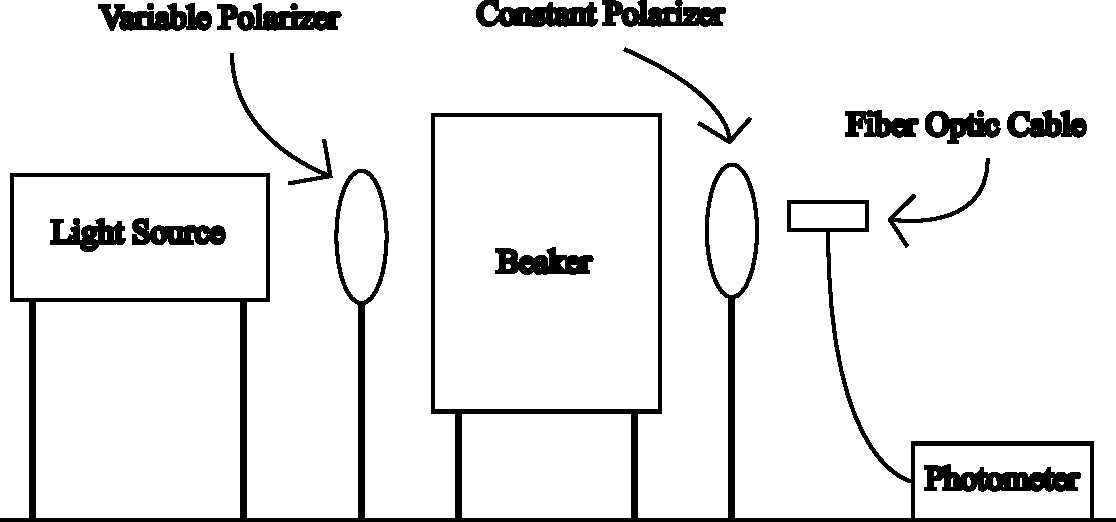
\includegraphics[scale=0.4]{../figures/setup.pdf}
\caption{The basic setup for measurements of both the polarization angle and intensity of light. The incident light enters the variable polarizer, refracts through the beaker, exits the constant polarizer, and finally is captured by the fiber optic cable, depositing a signal to the photometer.}
\end{figure}

% Uncertainties from measurements
The mass of sugar was measured using a scale with an uncertainty of $\pm 0.1$ grams. The volume of water was measured using a graduated cylinder with an uncertainty of $\pm 0.05$ milliliters (see Table \ref{tab:solution_concentration}). The diameters of the beakers were measured using a set of vernier calipers. More specifically, both the inside and outside diameters of each beaker was measured, and the final diameter was calculated using the average of the two measured diameters. This measurement provided an uncertainty of $\pm 0.1$ millimeters (see Table \ref{tab:beaker_diameters}). The uncertainty in measurement of both the polarization angle and the intensity contributed most of the measurement uncertainty in this experiment, with the polarization angle providing an uncertainty of $\pm 2$ degrees and the intensity with varying uncertainity values ranging from $\pm 0.01$ to $\pm 1$ arbitrary units (see Tables 3-8).

% Additional sources of uncertainty
There were several possible sources of uncertainty unrelated to error in measurement. The first was the use of external light sources. A phone flashlight was used to see the angle of the polarizer and the intensity meter in the dark room. Although the phone flashlight was necessary to make measurements, its effect on the intensity meter could have been minimized by shielding the fiber optic cable from the flashlight's light.
A secondary source of uncertainty could be the swirling of the solution in the beaker. The swirling solution occurred as a result of both heating and mixing the solution to ensure maximum dissolution of sugar. The swirling of the solution could have caused light to scatter unevenly, leading to either higher or lower intensity readings. The possible source of uncertainty stemming from the swirling of the solution could have been minimized by allowing the solution to settle longer prior to taking measurements.
A tertiary source of uncertainty could be the amount of light traveling through each differently sized beakers directly into the fiberglass optical cable. We are unsure if there would be any direct way to minimize the possible uncertainty stemming from the amount of light traveling through each differently sized beaker. However, this uncertainty can be disregarded when comparing intensity measurements between trials with the same beaker size, as the path length is the same for each measurement. A final possible source of uncertainty stemmed from the medium beaker being broken and needing to be replaced prior to the solution 2 experiment. Although unlikely, the replacement beaker could have had slightly different optical properties than the original medium beaker, potentially affecting the data trend.